%\documentclass[openright,twoside,headsepline]{scrbook}
%\usepackage[applemac]{inputenc}
%\usepackage{graphicx,xcolor,hyperref} % obsolete in HU-diss
%\usepackage[round,authoryear]{natbib}
%\setlength\bibhang{2em} 
%
%
%\KOMAoptions{numbers=noenddot}
\usepackage{amsmath,amssymb,amsfonts,amsthm,epigraph,scrpage2}
\usepackage[ngerman,english]{babel}
\definecolor{Cayenne}{rgb}{0.502,0.0,0.0}
\definecolor{Steel}{rgb}{0.4,0.4,0.4}


%\setcounter{secnumdepth}{3} % sub subsections numbering
%\setcounter{tocdepth}{3} % subsubsections inTOC

\usepackage[format=plain,singlelinecheck=false, font={sf,small},labelfont={bf,color=Steel}]{caption}
\DeclareCaptionLabelSeparator{cayenne_period}{\textcolor{Cayenne}{.} }
\captionsetup{labelsep=cayenne_period}

% Colors
\addtokomafont{chapter}{\color{Steel}}
\addtokomafont{section}{\color{Steel}}
\addtokomafont{subsection}{\color{Steel}}
\addtokomafont{subsubsection}{\color{Steel}}
\addtokomafont{paragraph}{\color{Steel}}

\addtokomafont{pagehead}{\color{Steel}}
\renewcommand{\pnumfont}{\color{Steel}} 
\addtokomafont{headsepline}{\color{Steel}} 
\pagestyle{scrheadings} 

%\makeatletter % dot after sections and all below
%\let\std@sect\@sect
%\def\@sect#1#2#3#4#5#6[#7]#8{\std@sect{#1}{#2}{#3}{#4}{#5}{#6}[#7.]{#8\color{Cayenne}{.}}}
%\makeatother

\usepackage[leftcaption]{sidecap} % inner, outer,left,right
\sidecaptionvpos{figure}{t}

% Papiergr��e
%\setlength{\paperwidth}{24cm}
%\setlength{\paperheight}{17cm}
%\recalctypearea
%\usepackage{geometry}

%% Flattersatz
%\usepackage[document]{ragged2e} % Flattersatz
%\setlength{\RaggedRightParindent}{1em} % evtl. parskip


%% Sans Serif
%\usepackage{cmbright}
%\renewcommand{\familydefault}{\sfdefault}
%% Palatino
%\usepackage[sc]{mathpazo}
%\linespread{1.05}         % Palatino needs more leading (space between lines)
%\setkomafont{sectioning}{\normalcolor\bfseries} % Kapitel�berschriften

%%% Kapitel�berschriften: Mit gro�en Zahlen
%\usepackage{titlesec}
%\titleformat{\chapter}[display]
%{\bfseries\Large}
%{ %\Huge\textsc{\chaptertitlename} % f�r das Wort 'Kapitel'
%\hfill\fontsize{120}{70}\selectfont\color{lightgray}\textbf{\thechapter}}
%{-2ex}
%%{\filleft\fontsize{50}{70}\selectfont\scshape} % Kapit�lchen oder...
%{\filleft\fontsize{50}{70}\selectfont\textbf} % ...oder keine Kapit�lchen
%[\vspace{0ex}]
%
%%%% Part�berschriften
%\titleformat{\part}[display]
%{\bfseries\Large}
%{ %\Huge\textsc{\chaptertitlename} % f�r das Wort 'Kapitel'
%\hfill\fontsize{120}{70}\selectfont\color{lightgray}\textbf{\thepart}}
%{-2ex}
%{\filleft\fontsize{50}{70}\selectfont\scshape} % Kapit�lchen oder...
%%{\filleft\fontsize{50}{70}\selectfont\textbf} % ...oder keine Kapit�lchen
%[\vspace{0ex}]


\newcommand{\ER}{Erd\H{o}s-R\'enyi }
\newcommand{\BA}{Barab\'asi-Albert }
\newcommand{\mean}[1]{\left< #1 \right>}
\newcommand{\abs}[1]{\left| #1 \right|}
\newcommand{\norm}[1]{\lVert#1\rVert}
\newcommand{\mat}[1]{\mathbf{#1}}
\newcommand{\tgraph}{\mathcal{G}}

\theoremstyle{definition} % non-italic
\newtheorem{annahme}{Annahme} % braucht amsthm
\newtheorem{definition}{Definition}
\newtheorem{theorem}{Theorem}
\newtheorem{satz}{Satz}
\newtheorem{frage}{Frage}
%\input{watermarks/watermark.tex}
\DeclareMathOperator{\nnz}{nnz}

% + Graphicspath nach begin document

%
%
%
%\begin{document}
%\graphicspath{{/Users/lentz/Documents/GitHub_locals/Thesis/images/}}
%\tableofcontents
%


\chapter{Theory}
This chapter is devoted to the mathematical formalism that is used to model infectious diseases and networks.
We define a mathematical framework and summarize relevant results of earlier research in this chapter.
In addition, section xx describes an efficient computer implementation of networks.

\section{Models of infectious diseases}
%\subsection{Very briefly:}
\paragraph{Main observations\color{Cayenne}{.}} Large scale patterns of epidemics have been measured \citep{giehl:2012}.
The spread of infectious diseases is something that everyone is familiar with.

\paragraph{Research field: Epidemiology\color{Cayenne}{.}} One goal of epidemiology is to understand the principles behind the spreading process, i.e. the way how a disease is transmitted through a population.
In this context, \emph{conceptional} models are used.
They make use of simple assumptions for the local (person-to-person) dynamics and focus on the big picture of the process.
Conceptual models are very similar to models in theoretical physics, because they focus on the very essence of the problem (here: the macroscopic view, spreading patterns).
However, they have to neglect many details of the real problem (here: physiology, symptoms, individual behavior, infection pathways and many more!) in order to have mathematical feasible models.

Another important issue of epidemiology is the \emph{forecast} of epidemic spreading processes.
Forecast models incorporate as much information as possible and the main focus is not an understanding of the basic principles.

This section summarizes the mathematical framework that roughly reproduces the behavior of infectious diseases and briefly discusses some major insights.

\subsection{Development of mathematical epidemiology}
The modeling of infection diseases mostly uses the concept of compartment models as explained in section xx.
Major contributions to the modern theoretical framework were provided by \citep{kermack:27}, \citep{bailey:57} and \citep{andersonmay:92}.
In his review about the mathematics of infectious diseases Hethcote reports a model for smallpox was already formulated in 1760 by D. Bernoulli (\citep{Hethcote:2000} and references therein).
In the early 20th century, people developed mathematical models for epidemics: a discrete time model in 1906 \citep{Hamer} and a differential equation model in 1911 \citep{Ross}.
The epidemic threshold (section \ref{sec:sir_model}) was found in the 1920s \citep{kermack:27}.
Starting from Bailey's book \citep{bailey:57} in the 1950s, the modeling of infectious diseases became a major scientific research field.
Modern models of infectious diseases include vaccination, demographic structure, disease vectors, quarantine and even game theory (\citep{Bauch:2004} and references in \citep{Hethcote:2000}).
The availability of contact data in recent years led to a strong impact on network analysis on epidemiology.
Well known concepts of mathematics (graph theory \citep{Bollobas:1985}) and social sciences (social network analysis \citep{WassermanFaust}) have been adopted to disease modeling, since the connections between individuals are related to their epidemic spreading potential \citep{Keeling:2005}.

\subsection{Infection dynamics}
The spread of infectious diseases can be modeled in terms of compartment models as described in sections \ref{sec:si_model} and\ref{sec:sir_model}.
We differentiate between \emph{conceptional models} and \emph{realistic disease models}.
While the former class is used to provide conceptual results as for the computation of thresholds or to test theories \citep{Hethcote:2000}, realistic disease models use as many aspects as possible to provide a forecast of the spreading process.
Realistic disease models can be very complex and are beyond the scope of this work, thus we focus on the use of conceptional models.
The following section is inspired by the Lecture notes of J.~R.~Chasnov \citep{Chasnov:2010}.

\subsection{SI model}\label{sec:si_model}
Let us consider a population of $N$ individuals.
In the simplest case, the infection status of each individual is either susceptible or infected and there are no births and deaths on the population.
Susceptible individuals become infected, if they are in contact with an infected.
In epidemiology, the classes susceptible and infected are called \emph{compartments} and every new infection increases the population of the infected compartment following the local reaction scheme
\[
S+I \rightarrow 2 I.
\]
This mimics the behavior of an infectious disease without immunization, i.e. infected individuals stay permanently infected.

Provided that $\alpha $ is the rate, under which new susceptible become infected, we obtain the differential equation model
\begin{align}\label{eq:si_model}
\frac{dS}{dt} &= -\alpha SI \nonumber \\
\frac{dI}{dt} &= \alpha SI,
\end{align}
where $S$ and $I$ are the numbers of susceptible and infected individuals respectively.
The model \eqref{eq:si_model} is called SI-model.
The total population is $N=S+I$.
Thus, \eqref{eq:si_model} can be rewritten as
\[
\frac{dI}{dt}=\alpha (N-I)I,
\]
i.e. a logistic differential equation.
Hence, in the limit $t\rightarrow \infty $ the whole population is infected ($I(\infty )=N$). 

\subsection{SIR model}\label{sec:sir_model}
In contrast of the infection dynamics introduced in the previous section, many epidemics allow for an immunization of the individuals.
Examples are measles or whooping cough \citep{grenfell:92} \citep{andersonmay:92}.
In this case, individuals recover from the disease after being infected for a certain time period, which is modeled by an additional compartment for the recovered population.
The infection scheme is extended to susceptible-infected-recovered (SIR) as in the following infection model \citep{kermack:27}:
\begin{align}\label{eq:sir_model}
\frac{dS}{dt} &= -\alpha SI \nonumber \\
\frac{dI}{dt} &= \alpha SI -\gamma I \nonumber \\
\frac{dR}{dt} &= \gamma I
\end{align}
where $\alpha $ is the infection rate and $\gamma $ is the immunization or recovery rate.
There is no analytic solution for the system \eqref{eq:sir_model}, but some fundamental conclusions can be obtained analytically.
We show a typical solution of \eqref{eq:sir_model} in figure \ref{fig:std_sir_model}.
%
\begin{SCfigure}%[htbp]
%\begin{center}
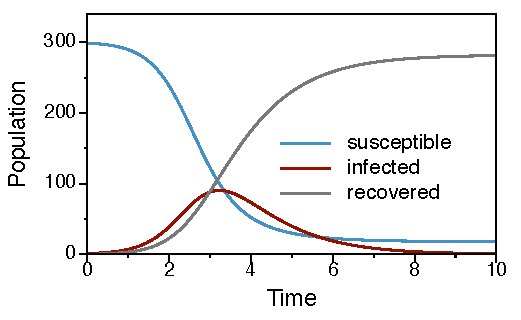
\includegraphics{sir_model.pdf}
\caption{Solution of the susceptible-infected-recovered (SIR) model \eqref{eq:sir_model}.
The number of infected shows that the spreading process is a single event.
Note that a fraction of the population is still susceptible at the end of the process.
Parameters: $\alpha = 3$, $\gamma = 1$, $N=300$, $S_0=1$.}
\label{fig:std_sir_model}
%\end{center}
\end{SCfigure}
%


The SIR model shows more sophisticated features than the SI model \eqref{eq:si_model}.
To begin with, we analyze the fixed points of the system, i.e. $(S_*,I_*,R_*)$ where
\begin{equation}
\frac{dS_*}{dt} = -\alpha S_*I_* =0 ,\; \;\;
\frac{dI_*}{dt} = \alpha S_*I_* -\gamma I_* =0,\; \;\;
\frac{dR_*}{dt} = \gamma I_* = 0.
\end{equation}
It follows from the last equation that $I_*=0$ at the fixed point, where $S_*$ and $R_*$ can be arbitrary.
Hence, a fixed point is $(S_*,0,R_*)$.

Let us analyze the stability of the fixed point in the early phase of an infection.
Almost all individuals are susceptible and consequently $I_*=N-S_*$.
An outbreak occurs, if and only if $dI/dt >0$ in this phase, i.e.
\begin{equation}\label{eq:prelim_condition}
\frac{dI}{dt}=\alpha S_* (N-S_*) - \gamma (N-S_*)=(N-S_*)(\alpha S_* -\gamma ) >0.
\end{equation}
It follows from \eqref{eq:prelim_condition} that the number of infected grows, if
\begin{equation}\label{eq:prelim_rnod}
\alpha S_* / \gamma >1.
\end{equation}
Equation \eqref{eq:prelim_rnod} is extremely important in epidemiology, because it defines a threshold for the unfolding of an infection spreading process.
We call this fraction the \emph{basic reproduction number} $R_0$.
Recall that $S_* \approx N$ in the fixed point.
Thus it follows that the outbreak condition is
\begin{equation} \label{eq:r0}
R_0 = N \frac{\alpha }{\gamma } >1.
\end{equation}

The basic reproduction number describes the average number of follow-up infections by each infected individual.
It is one of the main goals in epidemiology to bring down the basic reproduction number of a disease below the critical value $R_0=1$.
This is the reason for the implementation of mass vaccination.
As one can immediately see from equation \eqref{eq:r0}, this can be done by reducing the infection rate $\alpha $ or by increasing the immunization rate $\gamma $.
In principle, one could also reduce the size of the initial population $S_*$.
As an example, reducing the infection rate can be done by increasing hygiene standards or appropriate behavior, say wearing warm clothes in winter time to avoid common cold.
The immunization rate can be increased by vaccination.

Let us now focus on the late phase of an SIR-infection.
In contrast to the SI-model of section \ref{sec:si_model} an SIR like outbreak does not necessarily infect the whole population, even if $R_0>1$.
The reason is that there has to be a critical mass of susceptible individuals in order to keep an infection alive (see equation \eqref{eq:prelim_rnod}).
The total number of infected during an infection given by the number of recovered at the end of the infection, since every recovered has to be in the infected state in the first place.
A central measure throughout this work is therefore the \emph{outbreak size} $R_\infty$.

To compute the outbreak size, we consider the second fixed point of \eqref{eq:sir_model}, i.e. the fixed point for $t \rightarrow \infty $.
At this point there are no infected and a fraction of the population is recovered.
Hence the fixed point is $(N-R_\infty , 0, R_\infty )$.
A simple way to obtain the outbreak size $R_\infty $ is to use equations \eqref{eq:sir_model} and compute 
\[
\frac{dS}{dR}=-\frac{\alpha }{\gamma } S 
\]
and separate the variables \citep{Chasnov:2010}.
This yields
\[
\int _{S_*} ^{N-R_\infty} \frac{dS}{S}=-\frac{\alpha }{\gamma } \int _{R_*} ^{R_\infty} dR .
\]
We integrate from the initial condition at $t=0$ to the final condition at $t \rightarrow \infty$, where $S_\infty = N-R_\infty $.
Using that $R_* =0$ at $t=0$ gives 
\begin{equation}\label{eq:transcendental}
R_\infty = S_*-S_* e ^{-\frac{\alpha}{\gamma}R_\infty}.
\end{equation}
This transcendental equation can be solved numerically using a Newton-Raphson technique.
The outbreak size $R_\infty $ only takes finite values for $\alpha / \gamma > 1$.
A solution of equation \eqref{eq:transcendental} is shown in figure \ref{fig:transcendental}
%
\begin{figure}[htbp]
\begin{center}
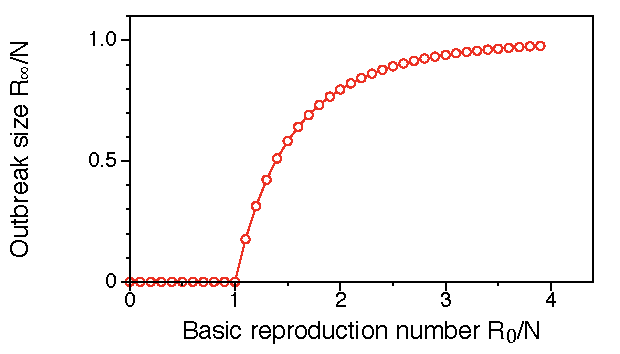
\includegraphics{R_0_R_infty.pdf}
\caption{Relative outbreak size vs. basic reproduction number.
The outbreak size takes finite values only for $R_0/N >1$.
Note that even for supercritical $R_0$ the outbreak size is in general smaller than the total population.
}
\label{fig:transcendental}
\end{center}
\end{figure}

It should be noted that an SIR epidemic is a single event, i.e. it possesses a \emph{characteristic time scale}.
The analysis of the late phase of an epidemic also gives information about these time scales.
Let us consider the second equation of \eqref{eq:sir_model}.
\begin{equation}\label{eq:sir_model_only_i}
\frac{dI}{dt} = \alpha SI -\gamma I
\end{equation}
In the late phase of an SIR-type epidemic, the fraction of infected is small.
Given sufficiently large values of $R_0$, the fraction of recovered is also small in this phase (see figure \ref{fig:transcendental}).
Thus, we neglect the quadratic term in \eqref{eq:sir_model_only_i}.
This gives $\frac{dI}{dt} = -\gamma I $, which has the solution
\[
I(t)=I(0)e^{-\gamma t}.
\]
Hence, the infection decays exponentially for large $t$ and the inverse recovery rate $1/\gamma $ defines the characteristic time of the epidemic.

A similar concept to the SIR model is the SIS model, where infected individuals return to the susceptible state after a certain period.
Being a single-event model, the SIS model has many similarities to the SIR model.
The most crucial difference is that SIS models show an endemic state for $t\rightarrow \infty $, i.e. both $S$ and $I$ take finite values in the long term.

\subsection{Force of infection}\label{sec:force_of_infection}
The model presented in section \ref{sec:sir_model} describes only the very basic behavior of epidemic dynamics, and is therefore a conceptual model.
However, it is one of the main objectives in epidemiology to have an understanding of the exact infection rates in the process.
Infection rates their selves can cause complex infection dynamics.

The term $\alpha I$ used in section \ref{sec:sir_model} is a special, very simple case of an infection rate.
More generally, we have to replace $\alpha I$ by an abstract infection rate $\lambda $ containing more information about the interaction between susceptible and infected individuals \citep{Keeling:2005}.
Thus, the equation for the infected becomes
\[
dI/dt = -\lambda S -\gamma I.
\]
The rate $\lambda $ is called the \emph{force of infection}.
In principle, this parameter can be arbitrarily complex, because it contains detailed information about the mixing properties of the population.
This information could be given as contact networks, demographic contact structures, etc.

In most cases, detailed information about mixing is not available.
Instead, we assume \emph{random mixing} of the population, i.e. every individual can be in contact with every other individual.
This yields a transmission rate \citep{Keeling:2005}
\begin{equation}\label{eq:force_of_infection}
\lambda = \tau n \frac{I}{N}\equiv \beta \frac{I}{N},
\end{equation}
where $\tau $ is the transmission rate, $n$ is the effective contact rate and $I/N$ is the fraction of infectious contacts.
It is therefore reasonable to replace the infection term $\alpha $ in \eqref{eq:sir_model} by $\beta /N$ to explicitly include the force of infection.
Nevertheless, the results presented in section \ref{sec:sir_model} remain qualitatively the same.

Although the force of infection gives a more reasonable description of the infection process, the assumption of random mixing remains inappropriate for many real world systems.
Due to the availability of contact data, the random mixing assumption can be improved in terms of contact networks.
Even if the exact data of an epidemic system is not available, research on complex networks allows us to give more realistic models about mixing.
In the next section, we briefly report important results in complex network research and focus on the interplay between networks and epidemics in section \ref{sec:epi_networks}.


\section{Network theory}\label{sec:network_theory}
As we have seen in the previous section, standard epidemic models make use of the random mixing assumption.
This assumption seems reasonable, if no further information about the contact structure within a population is available, because it gives a worst case scenario of the infection dynamics.
Even an overestimation of the outbreak size can be corrected by introducing smaller, effective disease parameters.
However, the random mixing assumption does not allow for non homogenous mixing, i.e. each individual is considered equal.
Nevertheless, the equality of individuals is not a reasonable assumption for many epidemic substrates.
Examples are contact structures of humans, livestock trade, vehicles as disease vectors of links between computers.

\paragraph{Main observations\color{Cayenne}{.}}
The random mixing assumption is obsolete in the vast majority of systems.
Instead, these systems possess an underlying contact structure -- a network.
Since the beginning of the 21st century, large amounts of data about these contact structures became available for social, economic, transportation and biological networks.
Observations showed that many real-world networks share common topological properties (see section \ref{sec:macro_measures}).
However, the number of their non-trivial topological properties is considerable, therefore they are often referred to as \emph{complex} networks.

\paragraph{Research field: network science\color{Cayenne}{.}}
Modern network science is an interdisciplinary research field, because it addresses systems of diverse scientific affinity.
Its roots lie in graph theory (mathematics) and social network analysis (social sciences).
Social network analysis plays a particular role for the definition of local network measures (see section \ref{sec:micro_measures}), whereas the influence of graph theory is stronger in macroscopic problems like percolation or graph partitioning.
An important focus of network science is to find common features of different networks and to find the basic principles behind their emergence.
Applied network science is often found in computer science.

\subsection{Matrix representations}\label{sec:network_matrices}
A network is a system consisting of nodes that are connected by edges.
Edges can be undirected, directed and weighted.
In principle, a network can consist of edges of different types.
This can be represented by multiple networks sharing the same set of nodes, but different edges.

Networks are called graphs in mathematical literature.
A graph $G=(V,E)$ is a set of nodes (or vertices) $V$ and edges (or arcs) $E$, where each edge is given by the tuple of nodes it connects, i.e. $e_1 =(u,v) \in E$ connects nodes $u$ and $v$.
An edge $(u,v)$ being present in an undirected network implies an edge $(v,u)$.
Apparently, this does not hold in directed networks.
Edges of weighted networks carry additional meta information about their weight.
This meta information can be their importance, capacity, number of transported items or the geographical distance between nodes $u$ and $v$.

Graphs can be represented by different graph matrices, where different matrix representation emphasize typical properties of the network.
The most common graph matrix is the \emph{adjacency matrix} $\mathbf{A}$ with entries
\begin{equation}\label{eq:adjacency_matrix}
a_{ij}\equiv (\mathbf{A})_{ij}= 
\begin{cases}
1 & \text{if $i$ is connected to $j$} \\
0 & \text{else.}
\end{cases} 
\end{equation}
An adjacency matrix contains the edges of the graph and can be seen of the most fundamental graph representation.
Figure \ref{fig:simple_digraph} shows a simple example of a directed graph and its adjacency matrix.
The corresponding matrix would be symmetric in the undirected case.
Weighted networks can be represented by weight matrices, where the values of the entries in \eqref{eq:adjacency_matrix} are not restricted to zero and one.
%
\begin{SCfigure}%[h]
%\begin{center}
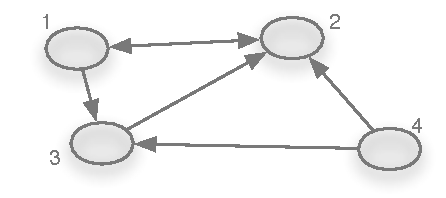
\includegraphics{Simple_DiGraph}
\caption[Adjacency matrix.]{A simple directed network. The corresponding adjacency matrix is
\[
\mathbf{A}=\left(\begin{array}{cccc}0 & 1 & 1 & 0 \\0 & 0 & 0 & 1 \\0 & 1 & 0 & 0 \\0 & 1 & 1 & 0\end{array}\right).
\]
}
\label{fig:simple_digraph}
%\end{center}
\end{SCfigure}

The adjacency matrix of an undirected network is symmetric, because every non-zero entry $a_{ij}=1$ implies an edge into the opposite direction, $a_{ji}=1$.
Entries on the main diagonal $a_{ii}$ correspond to nodes with self loops, i.e. nodes with edges pointing back to themselves.
The $i$-th row the adjacency matrix contains non-zero entries $a_{ij}=1$, whenever node $i$ is connected to node $j$.
Hence, every row can be interpreted as the neighborhood of one node.
This holds for undirected and for directed networks.
The columns of $\mathbf{A}$ give the same information as the rows.
In the directed case, however, rows contain the out-neighborhood of each node and columns contain the in-neighborhood, respectively.

Information about paths of a certain length can be obtained using the powers of the adjacency matrix.
The adjacency matrix gives information about the number of paths of length $1$ between node pairs.
Evidently, the number of paths of length $2$ between two nodes $i$ and $j$ is given by $(\mathbf{A}^2)_{ij}$.
This applies also to paths of arbitrary length $n$ using the elements of $\mathbf{A}^n$.

An important example for weighted network matrices is a \emph{Markov chain}.
A Markov chain is a random process without memory and with discrete state space and discrete time.
It is called time-homogenous, if the transition rates are constant.
Time-homogenous Markov chains can be represented as weighted networks and the corresponding weighted adjacency matrix is the \emph{transition matrix}.
Transition matrices are stochastic matrices, i.e. the elements of every row sum up to unity.
Each node represents a different state of the system and the edges are weighted with the probabilities to transition into other states adjacent to these edges.
It is obvious that a transition matrix representation is useful to describe random walks on networks.
An example of such a process is shown in figure \ref{fig:markov_chain}.
The underlying network represents a line of locations, where the drunkard can be located.
At every time-step there is a certain probability to move to another location.
%
\begin{SCfigure}%[htbp]
%\begin{center}
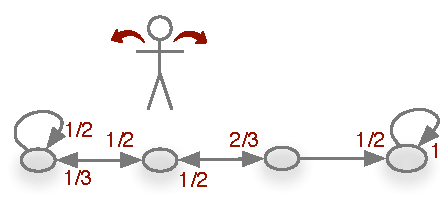
\includegraphics{Markov_chain.pdf}
\caption{Trajectory of a toddling drunk man as an example of a Markov chain.
At every location there is a probability for the drunkard to go left or right.
The node rightmost node is an absorbing state and could model a park bench.
Weights at arrowheads mark the transition probability.
(inspired by \citep{Aldous_book}).}
\label{fig:markov_chain}
%\end{center}
\end{SCfigure}
%
The state of the random walker can be described by a probability vector $\mathbf{p}$, where the initial state of figure \ref{fig:markov_chain} is $\mathbf{p}=(0,1,0,0)$.
The transition matrix $\mathbf{M}$ is a weighted adjacency matrix as it follows from the figure.
Given a state $\mathbf{p}_{t}$ at time $t$, the state of the next time step is given by $\mathbf{p}_{t+1}=\mathbf{p}_t \mathbf{M}^T$.
The equilibrium state $\mathbf{p}_\mathrm{eq}$ follows in the limit $\lim _{n\rightarrow \infty } \mathbf{p}_0 (\mathbf{M}^T)^n$, i.e. the equilibrium state is given by the dominant eigenvector of $\mathbf{M}$.

As a special case of transition matrices, the author would like to name the \emph{Google matrix}.
It describes a random walk on a network, but allows for shortcuts to any node in the network with a certain probability.
The eigenvectors of Google matrices are used for the computation of node rankings according to the PageRank-Algorithm \citep{PageRank:}.

Finally, the \emph{Laplace-matrix} of a network is an appropriate representation to model diffusion processes.
For undirected networks the Laplace-matrix is defined as
\begin{equation}\label{eq:laplace_matrix}
\mathcal{L}=\mathbf{D}-\mathbf{A},
\end{equation}
where $\mathbf{A}$ is the adjacency matrix and $\mathbf{D}$ is a diagonal matrix containing the degree $d_i=\sum _j a_{ij}$ of each node.
The definition \eqref{eq:laplace_matrix} has strong analogies to the discrete Laplace-Operator \citep{Press:1992}.
Consequently, they can be used to model diffusion processes on graphs in analogy to Laplace operators in continuous systems (see section \ref{sec:PRE}).

The spectra of adjacency and Laplace matrices contain information about the evolution/history of networks \citep{Banerjee2009}.


\subsection{Network measures}\label{sec:network_measures}
Before we address ourselves to models of real world networks, we have to introduce methods to measure structural properties of networks.
On the micro scale, this can be done in terms of \emph{node centrality} measures.
These measures are very important to assess the importance of single nodes in the network.
On the macroscopic side, we are interested in the large-scale properties of networks, i.e. percolation, distributions of centralities, connected components or other large scale structures.

\subsubsection{Network terminology}
Let $G=(V,E)$ be a graph consisting of a set of nodes $V$ and a set of edges $E$.
Every route across a graph along its edges without repeating nodes is called a \emph{path}.
Each path is given by an ordered set of the nodes traversed, i.e. $(v_1,v_2,\dots ,v_l)$, with $v_i \in V$ and all edges are in $E$, $v_i,v_{i+1} \subseteq E$.
If there is a path from every node in the network to any other node, the network is called \emph{connected}.
In directed networks, we have to consider two types of connectedness.
A directed network is strongly connected, if there is a directed path between all node pairs and weakly connected, if the node pairs would be connected ignoring the direction of edges.

The \emph{distance} between two nodes is the length of the shortest path between them and the longest distance is the \emph{diameter} of the network.
Every closed path is called a \emph{cycle}.
Graphs that do not contain cycles are called acyclic graphs or \emph{trees}.
The neighborhood of a node $u$ is the set of all nodes adjacent to it and the size of the neighborhood is the \emph{degree} of the node.
Hence, a node $v$ is in the neighborhood of $u$, if $(u,v) \in E$.
We distinguish between in-degree and out-degree in directed networks.
Finally, $G_0=(V_0,E_0)$ is a \emph{subgraph} of $G=(V,E)$, if $V_0 \subseteq V$ and $E_0 \subseteq E$.


\subsubsection{Microscopic measures}\label{sec:micro_measures}
Given a network, an important question is, if some nodes are more important as other nodes.
Therefore, we summarize measures of the \emph{centrality} of nodes.
The idea if centrality mainly goes back to social network analysis \citep{WassermanFaust,Freeman}, but has been widely adopted and extended in network science.
I restrict myself to those measures, that are indispensable when describing networks.
A more exhaustive overview of centrality measures is found in the review article \citep{MartinezLopez2009} or in online documentations of network analysis software, e.g.~\citep{hagberg2008,networkx:}.
In the following, $N$ denotes the order of the network (the number of nodes) and $m$ the number of edges.
%
\begin{figure}[htbp]
\begin{center}
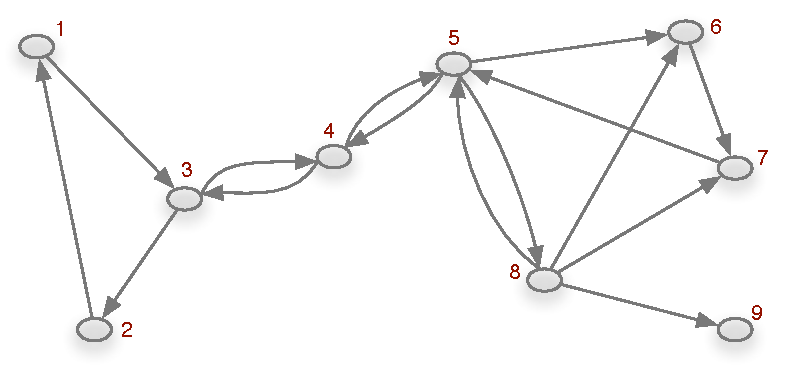
\includegraphics{DiGraph-Centrality}
\caption{A directed network for the demonstration of different centrality measures.}
\label{fig:example_net}
\end{center}
\end{figure}
%

\paragraph{Degree\color{Cayenne}{.}}
The simplest centrality measure is the degree $k$ of a node, which is the number of its neighbors.
In directed network, we distinguish between in-degree $k^-$ and out-degree $k^+$.
The degree follows immediately from the adjacency matrix, i.e.
\[
k ^-(i) = \sum _j a_{ji} \quad \text{and} \quad k ^+ (i)= \sum _j a_{ij}
\]
is the in- and out-degree of node $i$, respectively.
As an example, node $8$ in figure \ref{fig:example_net} has $k ^+(8)=4$ and $k ^- (8)=1$.
In weighted networks, the degree is computed in the same way and is called in-weight and out-weight of a node.

The degree centrality is used in a huge variety of applications.
One of its most important applications is to measure the heterogeneity of network connections, i.e. the existence of hubs in the network.
Hubs are nodes with a degree much larger than the rest of the system.
The heterogeneity of networks can be measured in terms of degree distributions (see section xx).


\paragraph{Closeness\color{Cayenne}{.}} 
The closeness of a node is the reciprocal average distance to all other nodes in the network.
It can be normalized, so that the closeness is $1$, if all other nodes are reachable within one step and $0$ in the limit of infinite distances to all other nodes.
The closeness of a node $i$ in a network of order $N$ is defined as follows:
\begin{equation}\label{eq:closeness}
c(i)=N-1 \sum _j \frac{1}{ d_{ij}}
\end{equation}
where $d_{ij}$ is the distance between nodes $i$ and $j$.
Some tools for an efficient computation of shortest-path distances are introduced in section \ref{sec:implementation}.
It should be noted that the distance between two nodes is defined to be infinite, if the underlying network is not connected.
In this case, the corresponding terms $1/\infty $ do not make contributions in equation \eqref{eq:closeness}.

The closeness centrality is capable to identify nodes with short average pathways to other parts of the network.
Identifying high closeness nodes is therefore reasonable for network navigation.
This holds in particular, if the exact route to the destination is unknown, because nodes with high closeness are probable to reach many destinations quickly.
In \citep{Zweig:closeness} it was shown that nodes of high closeness can act as landmarks for navigation.


\paragraph{Betweenness\color{Cayenne}{.}}
In order to identify nodes that act as bridges between two subgraphs, the measure of betweenness was developed.
In figure \ref{fig:example_net}, node $4$ plays such a role.
It is characteristic for these nodes to contain a relatively large number of shortest paths that have to cross them.
Therefore, betweenness of a node $i$ is defined as
\begin{equation}\label{eq:betweenness}
b(i)=\sum _{s\neq i \neq t} \frac{\sigma _{st}(i)}{\sigma _{st}}
\end{equation}
where $\sigma _{st}$ is the number of shortest paths between nodes $s$ and $t$ and $\sigma _{st} (i)$ is the number of shortest paths between $s$ and $t$ going through node $i$.
The computation of betweenness is expensive using equation \eqref{eq:betweenness}.
Therefore, an efficient algorithm was introduced by Brandes \citep{Brandes:2001p2757}.

Note that bridge nodes might look inconspicuous in the first place, e.g. they could have only two links.
Removing node $5$ in figure \ref{fig:example_net}, for instance, would divide the network into two disjoint subgraphs with nodes $V_1=(1,2,3)$ and $V_2=(5,6,7,8,9)$ respectively.
Therefore, removing nodes of high betweenness from the network has been proven useful in order to divide networks into smaller components \citep{girvan2002,Newman:2004}.


\paragraph{Eigenvector centrality\color{Cayenne}{.}}
The idea of eigenvector centrality can be easily realized by considering Markov chains as in section \ref{sec:network_matrices}.
Frequent multiplication of the transition matrix $\mathbf{M}$ with a random vector gives the largest eigenvector of $\mathbf{M}$.
This relation is known as power method or van Mises iteration \citep{van_mises}.
The dominant eigenvector of the transition matrix gives the equilibrium state of the system.
Using this state as a measure of centrality assigns every node with the probability to find a random walker here after a long period.
The principle behind the dominant eigenvector of an adjacency matrix $\mathbf{A}$ is that important nodes are likely to be connected to other important nodes.
This recursive concept is reflected in the equation
\[
x_i =\frac{1}{\lambda } \sum _j a_{ij} x_j ,
\]
where $x_i$ is the centrality of $i$, $\sum _j a_{ij} x_j$ is the centrality of the neighborhood of $i$ and $\lambda $ is a constant.
This equation can be rewritten as
\begin{equation}
\mathbf{Ax}=\lambda \mathbf{x}.
\end{equation}
It follows from the Perron-Frobenius-Theorem that $\lambda $ must be the largest eigenvalue of $\mathbf{A}$ in order to guarantee all entries of $\mathbf{x}$ to be positive \citep{Bonacich:1972,Bonacich:2007}.
The theorem guaranties unique solutions only to adjacency matrices of connected networks.
Hence, eigenvector centrality is only defined for connected graphs.
Nevertheless, the eigenvector centrality can be computed for each component separately, if a graph is not connected \citep{Bonacich:2007}.

Some important variants of eigenvector centrality are the PageRank and HITS algorithm \citep{Kleinberg:1999,PageRank:}.

\paragraph{Node components and range\color{Cayenne}{.}}
The component of a node is the set of nodes it is connected to by a path of any finite length.
We call the size of this set the \emph{range} of a node \citep{Lentz:2012pre}.
In directed networks, we distinguish between the out-component and in-component of a node.
The size of the former is its range and the size of the latter is its reachability.
Reachability measures the vulnerability of nodes against disease outbreaks in the network.
Given a network $G=(V,E)$ of $N$ nodes, the range of a node $v \in V$ is defined as
\begin{equation}\label{eq:range_def}
\mathrm{range}(v)=\frac{\left| \mathcal{N} \right| }{N}, \; \text{ where } \; \mathcal{N}=\{u \in V:\exists ( v\rightarrow u )\},
\end{equation}
where $ v\rightarrow u $ is a path from $v$ to $u$.
The reachability of a node is its range in the inverse graph $G^{-1}=(V,E^{-1})$, in which the directions of all edges are reversed. 

Apparently, the range of a node is of major importance for any epidemiological problem on a network, because it defines an upper bound for the size of any outbreak starting at this very node. 
Although the range measure is rather simple, it can show an interesting distribution.
The shape of its distribution is inherently related to percolation properties of the network (see section \ref{sec:network_analysis}).


\subsubsection{Macroscopic measures}\label{sec:macro_measures}
In order to get the big picture about a network, we discuss measures that capture large scale properties of networks.
The central question for the analysis of real-world networks is, whether different networks share similar large-scale features or whether each network is unique.
Is network=network\textbf{\textsf{\color{Cayenne}{?}}}

\paragraph{Degree Distribution\color{Cayenne}{.}}
In principle, the distribution of any centrality measure could yield insights into the macroscopic network structure.
As a matter of fact, the distribution of a networks degrees became a major criterium for the classification into different network types.
If all nodes of a graph have the same degree, the graph is called \emph{regular}.
Lattices are special cases of regular graphs.
In this case, the degree distribution collapses to a single peak without statistical variation.

Observations of real-world networks have shown that some networks exhibit exponential decaying degree distributions, i.e. there is a a variance of degrees, but the system possesses a \emph{typical degree}.
Examples are social networks and technological and economic networks, such as electric power-grids and traffic networks \citep{Amaral:2000,indian_railway}.

The nodes of the vast majority of large real-world networks, however, show a degree variation over several orders of magnitude.
Examples are the network of internet routers \citep{Faloutsos:1999}, www links \citep{Barabasi99} or scientific citations \citep{Price:1965}.
Their degree distributions are approximated by \emph{power-laws} of the form
\begin{equation}\label{eq:scale-free_distr}
P(k) \propto k^{-\gamma } ,
\end{equation}
where $2<\gamma <3$ for most observed networks \citep{all_scale_free_are_sparse,Newman2003}.
The approximation is reasonable for the tails of the distributions, i.e. for large values of $k$.
The identification of power-law distributions in data is discussed in \citep{Clauset:2009}.

Distributions of the form \eqref{eq:scale-free_distr} are called \emph{scale-free}, because they do not show a typical value (mean).
Instead, the network has nodes with only a few neighbors and hubs with very large degrees.
The structural difference between random and scale-free networks is sketched in figure \ref{fig:random_scalefree}.
%
\begin{figure}[htbp]
\begin{center}
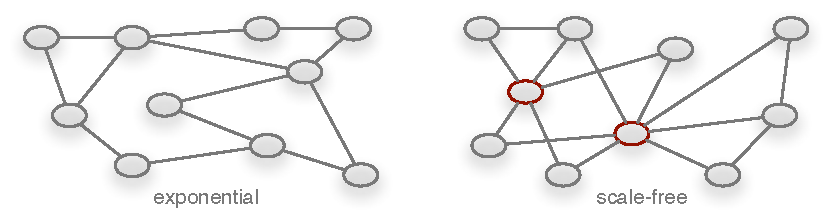
\includegraphics{exponential_scalefree}
\caption{Structural difference between networks with exponential and scale-free degree distributions.
All nodes have a similar degree in the random network, while the scale-free network shows hubs with a significantly larger degree than the average.
Hubs are highlighted in red.}
\label{fig:random_scalefree}
\end{center}
\end{figure}

Scale-free networks have attained remarkable attention in the last years and many real-world networks have been conjectured as scale-free \citep{Newman2003,Barabasi99}.
Important consequences of this classification were found to be a change in the threshold behavior of epidemic processes \citep{Pastor-Satorras_vespi:2001} and their topological resilience to node failures \citep{Albert:2000}.
The degree distributions of collaboration networks were well fitted by a scale-free distribution with a sharp cut-off \citep{Newman:2001p,Albert:2000}, i.e. $P(K)\propto k^{-\gamma }e^{-k/\kappa }$ with fitting constants $\gamma $ and $\tau $.
In \citep{Amaral:2000}, a possible explanation for the existence of an exponential cut-off was the aging of nodes, indicating that real systems possess a natural upper bound for their number of links.



\paragraph{Clustering coefficient\color{Cayenne}{.}}
The idea of the clustering coefficient comes from social networks.
It measures, whether a network contains a significantly large number of triangles.
This behavior is conjectured to be typical for social networks and has the simple meaning:
``a friend of your friend is likely to be your friend''.
The clustering coefficient $C$ is the number of connected triples ($A\rightarrow B \rightarrow C \rightarrow A$) divided by the actual number of triples ($A\rightarrow B \rightarrow C $) in the network.
Using the adjacency matrix $\mathbf{A}$, the clustering coefficient can be computed as follows:
\begin{equation}\label{eq:clustering_coefficient}
C=\frac{\operatorname{tr}(\mathbf{A}^3)}{\operatorname{sum} (A^2) -\operatorname{tr}(\mathbf{A}^2)},
\end{equation}
where $\operatorname{tr}(\mathbf{A} )$ denotes the trace of $\mathbf{A}$ and $\operatorname{sum} (\mathbf{A})=\sum _{ij} a_{ij}$ is the sum over all elements of $\mathbf{A}$.
In this work, we focus on the clustering coefficient as a macroscopic property of networks.
It should be noted that there is also a node clustering coefficient defined by $c_i=\sum _{jl} a_{ij}a_{jl}a_li/(k_i (k_i -1))$ \citep{Watts:1998,dynamical_processes}.
Thus, a network clustering coefficient can also be defined by the average $\mean{c_i}$, which however gives slightly different values as \eqref{eq:clustering_coefficient} and should not be mixed up with the latter.


The clustering coefficient plays an essential role in the small-world model of networks (\citep{Watts:1998}, section \ref{sec:network_models}) and has been found to be an important property not only in social networks \citep{Holland1971}, but in many real-world networks \citep{Newman2003}.

\paragraph{Average shortest path length\color{Cayenne}{.}}
The distance matrix $d_{ij}$ contains the distance between nodes $i$ and $j$ in the network.
Ignoring those node pairs with infinite distance (i.e. setting $d_{ij}=0$) gives the average shortest path length
\begin{equation}\label{eq:}
l=\frac{1}{N(N-1)}\sum _{i, j} d_{ij}
\end{equation}

It is a common feature of many networks that the average shortest path length is much smaller than the number of nodes in the network, i.e. typically networks contain shortcuts \citep{RevModPhys.74}.
An early and impressive example was shown by Milgrim, where the average distance between two randomly chosen people in the united states was measured to be 6 \citep{Milgram:1967}. 
This property is called \emph{small world} phenomenon.
It is an important building block of the Watts-Strogatz network model (\citep{Watts:1998}, section \ref{sec:watts_strogatz_model}).



\paragraph{Connected components\color{Cayenne}{.}}
A connected component $G_\mathrm{cc}=(V_\mathrm{cc},E_\mathrm{cc})$ is a subgraph of graph $G=(V,E)$, where there is a path between any node pair in $V_\mathrm{cc}$.
In directed graphs, connected component in the sense above is called \emph{strongly connected}.
A component is called \emph{weakly connected}, if it is connected ignoring the direction of edges.
Many real-world networks contain one \emph{largest connected component} (LCC) that is typically much larger than all other components of the system.
This component is therefore called \emph{giant component}.

In fact, the emergence of a giant component in a network is a 2nd order phase transition and is a graph theoretical percolation process \citep{Newman2003}. 
Components play an important role for epidemic processes, because the component membership of each node defines the maximum outbreak size of any epidemic started at this very node.
In the directed case, maximum outbreak sizes are bounded by the underlying strongly connected component (lower bound) and the out component of the starting node (higher bound).
The general component structure of directed networks is discussed in \citep{Dorogovtsev:2001jd} and we provide further discussion of their epidemiological relevance in section xx.


\paragraph{Accessibility\color{Cayenne}{.}}
If we directly connect each node of a network with all other nodes it is connected to by a path of whatever length, we get the \emph{accessibility} of the network.
Accessibility measures the ability of each node to reach destinations, which is in particular important for transportation systems \citep{Garrison:1960up}.
Mathematically, we define the accessibility graph (also \emph{transitive closure}) of a network as follows:
Let $G=(V,E)$ be a network.
Than $G^*=(V,E^*)$ is the accessibility graph of $G$ with $(u,v) \in E^*$, if there is a path from $u$ to $v$.
The accessibility graph is typically dense, because it contains many more edges than the underlying network.
In mathematical literature accessibility is called \emph{transitive closure} of a network.
A (weighted) adjacency matrix $\mathbf{C}$ of $G^*$ for a $N$-node network is given by the cumulative matrix
\begin{equation}\label{eq:cumulative_matrix}
\mathbf{C}= \sum _{i=1} ^{N-1} \mathbf{A}^i,
\end{equation}
where $\mathbf{A}$ is the adjacency matrix of $G$ and the elements of $\mathbf{C}$ contain the actual number of paths between each node pair.


\section{Network models and epidemiology}\label{sec:network_models}
The analysis of real-world networks in terms of the measures introduced in section \ref{sec:network_theory} has given useful insight into the structural properties of these systems.
In particular, observations showed that many networks have heavy-tailed degree distributions and show non vanishing clustering coefficients.
In this section we summarize the results of some widely used network models.
Being very essential models, the network models in this section are entirely defined by their degree distributions.
They are therefore generic realizations of ensembles with fixed $P(k)$.
At the end of the section, we give a comparison between the different models an discuss their relevance in epidemiology.

\subsection{Lattice model}
Lattice models are inherently related to homogeneously distributed geographical positions of individuals.
They show a high degree of regularity and their potential for SIS and SIR spreading processes has been studied in \citep{Harris:1974} and \citep{Bak:1990}, respectively.
The impact of the heterogenous susceptibilities has been studied in \citep{Sander2002293}.
It was found that this heterogeneity introduces a broadening of the critical region and the outbreak threshold can be increased in the case of heterogenous susceptibilities.


\subsection{Erd\H{o}s-R\'enyi model}\label{sec:er_model}
The Erd\H{o}s-R\'enyi model makes use of probabilistic methods to analyze network properties and is therefore a random graph model.
A \emph{random network} is generated by generating a set of $N$ nodes and connect each of the $\frac{1}{2}N(N-1)$ possible node pairs\footnote{We focus on undirected networks here. In the directed case, there are $N(N-1)$ possible node pairs.} with a certain probability $p$.
Networks generated this way are often called $G_{N,p}$ networks, although they are actually elements of a $G_{N,p}$ \emph{ensemble}\footnote{An equivalent approach is to consider a fixed number of edges $m$ instead, yielding a $G_{N,m}$ ensemble.}.

Random graph theory addresses questions about typical properties of networks with $N\rightarrow \infty $ nodes.
Consequently, the edge occupation probability $p$ is the key parameter in random graph theory.
Properties of particular interest are the average shortest path length or the distributions of degrees, component sizes (percolation) and the occurrence of special subgraphs such as triangles.
Apparently, the expected number of edges in the network is $\mean{E}=\frac{1}{2}pN(N-1)$, if $p$ is the edge occupation probability.
In addition, every edge increases the degree of two vertices, so that the \emph{average degree} of a random network of $N$ nodes is
\begin{equation}\label{eq:mean_er_degree}
\mean{k}=\frac{2\mean{E}}{N}=(N-1)p\simeq pN .
\end{equation}
In the directed case, we would get the same result for both, in degree and out degree, since the factors $2$ and $\frac{1}{2}$ would just disappear in \eqref{eq:mean_er_degree}.
It should be noted that the mean degree is the most appropriate parameter for the analysis of random graphs.
Equation \eqref{eq:mean_er_degree} demonstrates that the system behavior for each value of $p$ depends on the system size.

We obtain the \emph{degree distribution} of $G_{N,p}$, if we realize that the probability to find a node with degree $k$ is equal to the probability to find a node that is connected to $k$ other nodes, but not to the $N-k-1$ remaining nodes in the network.
Thus, the degree distribution is given by a bimodal distribution
\begin{equation}\label{eq:bimodal}
P(k)= \left(\begin{array}{c}N-1 \\k\end{array}\right) p^k (1-p)^{N-k-1} .
\end{equation}
Provided that we are interest in large networks ($N\rightarrow \infty $), equation \eqref{eq:bimodal} is approximated by a Poisson distribution, 
\begin{equation}\label{eq:poisson_distribution}
P(k) =\frac{\mean{k}^k }{k!} e^{-\mean{k}}
\end{equation}
i.e. there is variation in the degrees, but there still remains a \emph{typical degree} in the system.

It is an interesting feature of random graphs that for different edge occupation probabilities they show different phases.
For low values of $p$, nodes tend to form small connected components, whereas for increasing $p$ suddenly a \emph{giant component} emerges.
This giant component contains almost all nodes of the network.
The behavior for large values of $p$ has first been studied by Erd\H{o}s and R\'enyi \citep{ER:1959}.
A few years later, Erd\H{o}s and R\'enyi found thresholds for the emergence of subgraphs and a giant connected component \citep{ER:1960,ER:1961}.
Results for the occurrence of different subgraphs are summarized in \citep{RevModPhys.74}.

The size of the giant component and the mean component size can be computed analytically for random networks.
Following Newman \citep{Newman2003}, we observe that the probability that a node is in the giant component is equivalent to the probability that none of its neighbors are part of the giant component.
This probability is given by $u^k$, if $u$ is the fraction of nodes that are not in the giant component, i.e. $u$ is the probability that a randomly chosen node is not in the giant component.
An expression for $u$ can be obtained by averaging $u^k$ over all degrees $k$.
The degree distribution is given by \eqref{eq:poisson_distribution}.
Hence, the fraction of nodes not in the giant component is
\[
u=e^{\mean{k}(u-1)}.
\]
The size of the giant component is $S=1-u$ and consequently
\begin{equation}\label{eq:giant_component}
S=1-e^{-\mean{k}S}.
\end{equation}
One can use similar arguments to obtain an expression for the mean cluster size \citep{Newman2003}
\begin{equation}\label{eq:mean_cluster_size}
\mean{s}=\frac{1}{1-\mean{k}+\mean{k}S}.
\end{equation}
%
The largest connected component phase transition is shown in figure \ref{fig:ER_lcc_emergence}.
\begin{SCfigure}
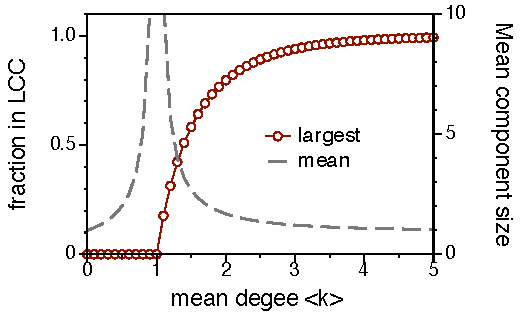
\includegraphics{ER_emergence_LCC.pdf}
\caption{Emergence of the largest connected component (LCC) in an \ER graph as it follows from \eqref{eq:giant_component}
The size of the of the largest component takes finite values for $\mean{k}>1$.
The mean cluster size is given by equation \eqref{eq:mean_cluster_size} and diverges at $\mean{k}=1$.
}
\label{fig:ER_lcc_emergence}
\end{SCfigure}
%

Since all edges in a random network are independent and identically distributed, the probability that a given node is part of a connected triple is $p^2$.
In analogy, the probability that a given node belongs to a closed triangle is $p^3$.
Consequently, the \emph{clustering coefficient}  \eqref{eq:clustering_coefficient} of a $G_{N,p}$ network is given by
\begin{equation}\label{eq:er_clustering}
C=\frac{p^3}{p^2}=p=\frac{\mean{k}}{N}.
\end{equation}
Equation \eqref{eq:er_clustering} shows that the clustering coefficient of random graphs vanishes in the limit of large networks.
We end this section by giving an approximation of the average shortest path distance in random graphs. 
Starting at some node in the network, the average number of nodes at distance 1 is given by the mean degree $\mean{k}$. 
Hence, the average number of neighbors at distance $d$ is $\mean{k}^d$.
In order to reach all $N$ nodes in the network, we need $r$ steps, where $r$ is determined by $\mean{k}^r\simeq N$.
Thus, $r$ approximates the diameter of the network.
Since we are only interested in the rough behavior of the average shortest path length $\mean{l}$, we approximate it by $r$ \citep{dynamical_processes} and obtain 
\begin{equation}\label{eq:er_av_shortest}
\mean{l}\simeq \frac{\log N}{\log \mean{k}}.
\end{equation}
The average degree remains constant for different network orders, so that equation \eqref{eq:er_av_shortest} demonstrates that the average shortest path length grows logarithmically with the number of nodes in \ER graphs.
This relation is found in many complex networks and is an indication for the small-world effect introduced in the next section.

\subsection{Watts-Strogatz model}\label{sec:watts_strogatz_model}
We have seen that random graphs can reproduce some important properties of real-world networks, particularly the existence of a giant component and small average shortest path length.
Nevertheless, equation \eqref{eq:er_clustering} demonstrates that the tendency to form connected triangles is absent in large scale \ER networks.
Observations show, however, that many real-world networks show this feature \citep{WassermanFaust,Newman2003,Milgram:1967}.
It is characteristic for social networks in particular to have a high degree of clustering and at the same time short-cuts allowing for small average shortest path distances.
In this sense they can be seen as an intermediate structure between lattices (high local order) and random graphs (small shortest path distances).
Therefore, Watts and Strogatz introduced the \emph{small-world model} in 1998 \citep{Watts:1998}.
We briefly summarize some of its main findings.

A Watts-Strogatz model interpolates between lattices and random networks by rewiring edges of a lattice.
We start with a regular ring lattice of $N$ nodes, where each node is connected to $m$ of its nearest neighbors on the lattice.
Then, each edge is rewired randomly with probability $p$.
Keeping $m$ constant from the beginning yields a scalable topology for different values of $p$.
The clustering coefficient $C$ and the average shortest path length $\mean{l}$ for different values of $p$ are shown in figure \ref{fig:watts_strogatz}.
Both values are normalized by their corresponding values in the initial lattice, i.e. $C/C_0$ and $\mean{l}/\mean{l}_0$ respectively.
%
\begin{SCfigure}
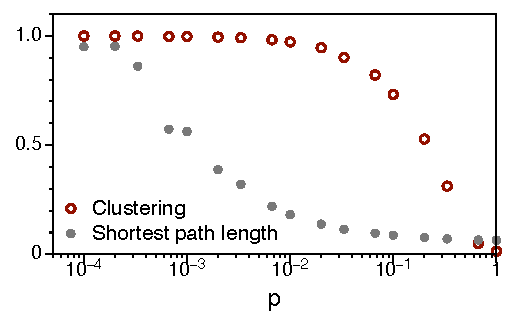
\includegraphics{Watts_strogatz.pdf}
\caption{Clustering coefficient and average shortest path length in the Watts-Strogatz model.
Both quantities are  normalized to the the corresponding value for $p=0$.
Results for networks with $N=1000$ nodes and $m=10$.
Every data point is the average of 1000 realizations.}
\label{fig:watts_strogatz}
\end{SCfigure}

The degree distribution collapses to a single peak for $p=0$.
In their paper about properties of small-world networks \citep{Barrat:2000fj}, Barrat and Weigt showed that the distribution converges to a Poisson distribution in the limit $p\rightarrow 1$ and found an analytical approximation for the clustering coefficient for different values of $p$.
The percolation threshold of small-world networks was investigated in \citep{Sander2002293}, where the authors found the threshold to be reduced for increasing values of $p$.

There is no sharp criterion for a network to be called small-world network.
Instead, a network is called small-world network, if it shows a sufficiently large clustering coefficient \emph{and} a sufficiently low average shortest path length.
This is the intermediate region in figure \ref{fig:watts_strogatz}. 

\subsection{Barab\'asi-Albert model}
Besides the critical behavior in \ER networks and the small-word effect in Watts-Strogatz networks, observations of real networks showed that they possess heavy-tailed degree distributions \citep{Barabasi99,Liljeros:2001p841}.
A central question is, where such distributions originate from.
Therefore, Barab\'asi and Albert introduced a network model in order to mimic the evolution of the world wide web \citep{Barabasi99}.
The system under consideration is a network of websites (nodes) that are connected by hyperlinks (edges) and should not be confused with the physical network of internet routers.
The evolution of the www-network is reduced to two simple principles.
(1) new nodes are added to the system over time and (2) the new nodes have a higher probability to link to existing nodes of higher degree.
The second principle can be summarized as a rich-get-richer phenomenon, i.e. the more links you have the more you will get.
In network language, this mechanism is called \emph{preferential attachment}.
It can be seen as the network version of what is also known as Matthew-effect or cumulative advantage \citep{Merton:1968fh,price:1976}.

The preferential attachment model for growing networks is as follows:
Start with a small number $m_0$ of nodes and add a new node at every time step.
Connect the new node to $m<m_0$ existing nodes, each with probability $\Pi $.
Thus, $m=1$ yields a tree and $m>1$ gives a graph with cycles.
The probability for an existing node $i$ to be connected with the new one depends on the degree of $i$, i.e. $\Pi (k_i)=k_i/\sum _j k_j$.
\begin{SCfigure}
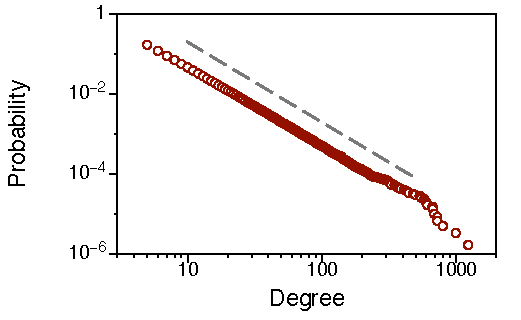
\includegraphics{BA_graph.pdf}
\caption{Cumulative degree distribution of a \BA graph with $N=10^5$ nodes and $m_0=m=5$.
The dashed line shows a power-law $P(k)\propto k^{-2}$.}
\label{fig:BA_cdf}
\end{SCfigure}

Figure \ref{fig:BA_cdf} shows the degree distribution of a network generated this way.
We have to point out that it is generally more appropriate to plot the cumulative distribution of such distributions, because it is more robust against statistical fluctuations, particularly in the tail of the distribution \citep{Clauset:2009}.
As the figure shows, the distribution is well approximated by a power law of the form
\[
P(k)\propto k^{-\gamma }
\]
with $\gamma =2$ for the cumulative distribution and $\gamma = 3$ for the probability density function, respectively.

Barab\'asi and Albert could show analytically that the resulting network has a power-law degree distribution of the form
\begin{equation}\label{eq:BA_law}
P(k)=2m^2 k^{-3}.
\end{equation}
Although the slope $\gamma = 3$ does not match the power-law exponent of the world wide web ($\gamma = 2.1\pm 0.1$ \citep{Barabasi99}) the model explains the existence of a scale-free degree distribution.

As a conceptual model, the \BA model has a huge field of applications for theoretical questions.
Nevertheless, the power-law degree behavior is also reproduced by fitness models \citep{Bianconi:2001,Fortunato:2006} and copy models \citep{Kleinberg99theweb}.
Fitness models allow for higher flexibility in terms of the power-law exponent.
However, the range of possible exponents cannot take values in the interval $0<\gamma < 2$ \citep{all_scale_free_are_sparse}.

Besides the models discussed above, there are other network models, such as the configuration model or exponential network models. 
The \emph{configuration model} is a more sophisticated random graph model that allows for arbitrary degree distributions \citep{Newman:book,Newman:2001pa}.
Moreover, the degree sequence of a given network remains constant.
In the configuration model one can consider higher order statistics, such as degree correlations and the clustering coefficient.
\emph{Exponential random graphs} are related to the concept of the micro canonical ensemble in statistical mechanics \citep{Strauss:86}.
In this context, an \ER graph is just one realization of an ensemble of possible random graphs.
Exponential random graphs are an elegant way of treating networks, but their mathematical treatments appears intractable for many cases of interest \citep{Newman2003}.

\subsection{Resilience of different network types}\label{sec:resilience}
A fundamental difference between complex networks and man made technological systems is their robustness against failure.
Failure can be modeled by \emph{randomly} removing nodes of the system\footnote{Removing edges instead of nodes gives similar results.}.
In this sense, network failure can be seen as an inverse percolation problem.
The degree of failure is then given by the fraction of removed nodes $f$ and the sensitivity of a network to random failure can be measured in terms of the size of its largest connected component, which is inherently related to its functionality.
As an example, if only a few circuits in a computer would randomly fail, the largest connected component would disintegrate into smaller circuits and the machine is likely to not function any more.
It is characteristic for complex networks, however, that randomly removing vertices does not drastically change the connectivity of the network.
The effect of network failure for different network types has been measured in \citep{Albert:2000}.
The authors found that \ER networks are more prone to random failure than scale-free networks.
The robustness of scale-free networks against random node removal is explained by the huge number of low-degree nodes in the network, so that it is unlikely to remove a hub at random.

The situation changes dramatically, when nodes are not removed at random, but targeted, i.e. the most central nodes are removed first.
This procedure models aimed \emph{attacks} on the network.
\citeauthor{Albert:2000} found that scale-free network are extremely vulnerable to attack of the most central nodes.
Figure \ref{fig:robustness} shows the size of the largest connected component (LCC) vs. the fraction of removed nodes for an \ER network and a scale-free \BA graph.
%
\begin{SCfigure}
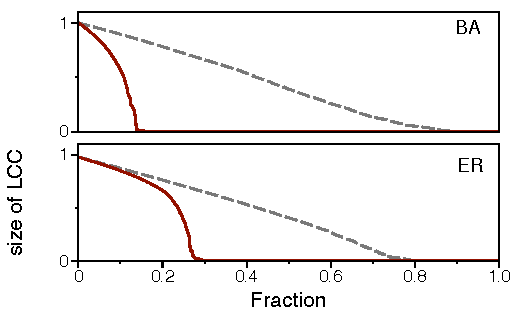
\includegraphics{Robustness.pdf}
\caption{Robustness of a \BA  (BA) network and an \ER  (ER) graph to random failure (grey dashed line) and targeted attack (red).
Red lines represent the size of the LCC under targeted removal of the most connected nodes.
The size of the LCC remains finite for the \BA network under random failure even for a large number of removed nodes.
From \citet{Albert:2000}.
}
\label{fig:robustness}
\end{SCfigure}
%
The figure shows results for a \BA network with $m=2$ and a \ER network with $p=0.0004$ at the beginning.
Both networks have $10^4$ nodes.
Note that the \BA network does not show a finite threshold for random node removal as the \ER network.
Thus, the network shows finite connected components even if a very large number of nodes has been removed from the network.
The robustness against random removal comes at the price of high vulnerability against removal of the most connected nodes (red lines).
After removing a relatively small fraction of high-degree nodes, the \BA network disintegrates into small components.

A different measure of integrity of a network is how the diameter changes when nodes are removed at random or after a certain criterion.
The differences between random and scale-free networks remain similar in this perspective.
In addition, the definition of a targeted attack can be extended to any centrality measure.
Although many centrality measures correlate in many network models \citep{dynamical_processes}, different attack strategies may be effective in real networks \citep{holme:2002}.

\subsection{Epidemics on networks}\label{sec:epi_networks}
The spread of infectious diseases on networks is substantially related to network resilience.
As we have seen in section \ref{sec:sir_model}, individuals are removed from the population in an SIR-type disease.
This corresponds to the failure of nodes as discussed previously.
Moreover, results from attacking networks can be carried over to vaccination strategies.
The central subjects of interest remain the same as in section \ref{sec:sir_model}, namely the epidemic threshold $R_0$ and the outbreak size $R_\infty $.

We have seen in sections \ref{sec:si_model} and \ref{sec:sir_model} how epidemics can be modeled under the assumption of homogenous mixing of individuals.
Nevertheless, data sources are available allowing for a more detailed analysis of an epidemic spreading process.
We start by considering the network models as introduced in section \ref{sec:network_theory} and summarize results about the impact of different topologies on spreading processes.

\paragraph{Epidemic models on homogenous contact networks\color{Cayenne}{.}}
To begin with, we consider a 2-compartment SI-model on a network of $N$ individuals, where a fraction $i(t)=I(t)/N$ individuals are infected and the remaining fraction $s(t)=1-i(t)$ is susceptible.
The force of infection (\eqref{eq:force_of_infection} in section \ref{sec:force_of_infection}) models the effective interaction between susceptible and infected individuals in terms of passing on the infection.
In a homogenous network, e.g. an \ER or Watts-Strogatz network, the force of infection is $\lambda = \beta ki$, where $ki$ is the number of infectious contacts for a node of degree $k$ and $\beta $ is the probability of infection per time unit \citep{dynamical_processes}.
Consequently, $1/\beta $ is the spreading time scale of the process.

In order to obtain a rate-equation for the total number of infected in a homogenous network, we replace the local degree $k$ by the mean degree $\mean{k}$ and get
\begin{equation}\label{eq:si_network}
\frac{di(t)}{dt}=\beta \mean{k} i(t) [1-i(t)],
\end{equation}
where $1-i(t)$ is the fraction of susceptible nodes.
This model can easily be extended to a SIS model by adding a loss term $-\gamma i(t)$ to equation \eqref{eq:si_network}.
Setting $\gamma =1 $ without loss of generality, we obtain 
\begin{equation}\label{eq:sis_network}
\frac{di(t)}{dt}=-i(t)+ \beta \mean{k} i(t) [1-i(t)] .
\end{equation}
The behavior of the SIS-model has been studied for Watts-Strogatz and \BA networks in \citep{Pastor-Satorras_vespi:2001}.
Following \citeauthor{Pastor-Satorras_vespi:2001}, we compute the steady state of \eqref{eq:sis_network} in order to find the epidemic threshold (see section \ref{sec:sir_model}), that is
\[
i[-1+\beta \mean{k} (1-i)]=0.
\]
$\beta $ being fixed as a local reaction constant, the average degree $\mean{k}$ remains the only parameter in this equation.
We define the critical connectivity $\beta _c=\mean{k}^{-1}$ and obtain distinct regimes for different values of $\beta $.
Thus, the density of infected in the endemic state is
\begin{align}\label{eq:endemic_ws}
i&=0   &\text{if} \quad \beta < \beta _c \nonumber \\
i &=1-\frac{\beta _c}{\beta }  &\text{if} \quad \beta > \beta _c .
\end{align}

This shows that the threshold behavior (see section \ref{sec:sir_model}) found for homogeneously mixed populations remains unchanged for homogenous networks.
In fact, is has been shown that homogeneously mixed epidemic models can always be mapped onto a percolation process on a regular lattice   \citep{Grassberger1983157,Sander2002293}.

\paragraph{Impact of heterogenous connectivity\color{Cayenne}{.}}
In order to consider networks with heavy-tailed degree distributions, we modify the SIS model above and include the heterogeneity of node degrees explicitly \citep{Pastor-Satorras_vespi:2001}.
\citeauthor{Pastor-Satorras_vespi:2001} replaced the infected compartment $i(t)$ by the fraction of infected with a given degree, that is $i(t)\rightarrow i_k(t)$.
The average degree in \eqref{eq:sis_network} is replaced by the actual degree and the force of infection is extended by the probability $\Theta (i(t))$ that a given link points to an infected node.
The latter depends on the total density of infected and it depends only on $\beta $ in the steady state.
This gives the following SIS model for heterogenous networks:
\begin{equation}\label{eq:sis_het_network}
\frac{di_k(t)}{dt}=-i_k(t)+\beta k [1-i_k(t)] \Theta (i(t)).
\end{equation}
%
\begin{SCfigure}
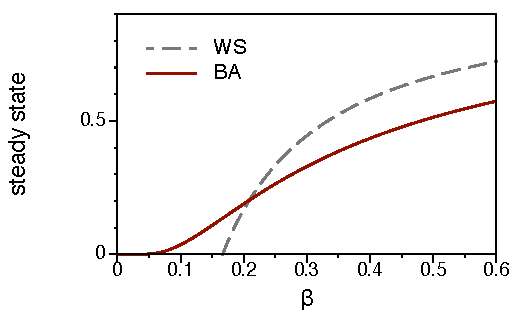
\includegraphics{Pastor-Satorras.pdf}
\caption{Fraction of infected in the endemic state for an SIS model.
The figure reveals the disappearance of the epidemic threshold for in \BA networks (red).
The epidemic threshold remains finite (here: $\beta _c=1/6$) for homogenous networks and $\beta _c \rightarrow 0$ for \BA networks.
From \citet{Pastor-Satorras_vespi:2001}.
}
\label{fig:pastor-sat}
\end{SCfigure}

%
\citeauthor{Pastor-Satorras_vespi:2001} found an analytic expression for the steady state by using statistical arguments to obtain an expression for $\Theta (\beta )$.
After some calculations, the density of infected in the endemic state for a \BA network with average degree $m=k/2$ reads
\begin{equation}\label{eq:endemic_ba}
i \sim e^{\frac{-2}{\mean{k}\beta }}
\end{equation}
and the condition for the epidemic threshold is \citep{pastor-sat_2}
\begin{equation}\label{eq:degree_threshold}
\beta _c=\frac{\mean{k}}{\mean{k^2}} .
\end{equation}
A graphical comparison between \eqref{eq:endemic_ws} and \eqref{eq:endemic_ba} is given in figure \ref{fig:pastor-sat}.
It is an important result that the epidemic threshold vanishes in \BA networks.
As a consequence, random vaccination in \BA networks does not suppress a disease outbreak \citep{Keeling:2005}.
Nevertheless, figure \ref{fig:pastor-sat} shows that for the outbreak size remains small for $\beta \rightarrow 0$.
Finally, the absence of the epidemic threshold is generally found in infinite scale-free networks with degree distributions $P(k)\sim k^{-\gamma }$ for $2\leqslant \gamma \leqslant 3$.
It should be noted that a geographically embedded network with the same degree distribution can still show a finite outbreak threshold \citep{Sander20031}.

\paragraph{Vaccination strategies\color{Cayenne}{.}}
As we have seen in the previous section, random immunization fails in scale-free networks, because it gives the same priority to low degree nodes and large hubs, while large hubs are unlikely to be chosen by chance.
Random immunization effectively reduces the infection rate $\beta \rightarrow \beta (1-g)$, where $g$ is the fraction of vaccinated nodes.
Therefore, the epidemic threshold condition \eqref{eq:degree_threshold} reads $\beta (1-g_c)=\mean{k}/\mean{k^2}$ with the critical immunization density $g_c$.
It follows
\begin{equation}\label{eq:critical_vacc}
g_c=1- \frac{1}{\beta } \frac{\mean{k}}{\mean{k^2}}.
\end{equation}
Given a scale-free network with diverging $\mean{k^2}$, the total population has to be vaccinated in order to drop the infection rate below the epidemic threshold.

Nevertheless, scale-free networks are vulnerable to targeted removal of highly connected nodes (see section \ref{sec:resilience}).
Immunization of the mostly connected nodes is therefore an effective vaccination strategy on these networks.
Numerical results for different vaccination strategies applied to a SIS-disease in a \BA network are shown in figure \ref{fig:targeted_immunization}.
%
\begin{SCfigure}
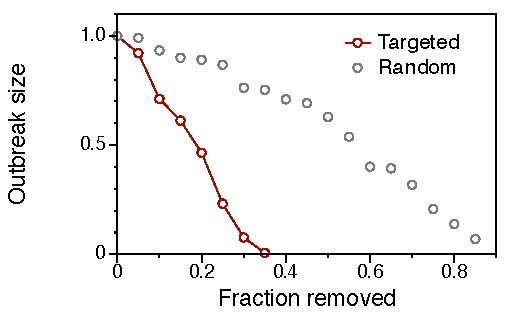
\includegraphics{SIS-Vacc.pdf}
\caption{Targeted and random vaccination for an SIS disease in a \BA network with $10^5$ nodes and $m=4$.
Infection parameters $\beta / \mu =2$.}
\label{fig:targeted_immunization}
\end{SCfigure}
%

In analogy to \eqref{eq:critical_vacc}, an analytic expression for the critical immunization density can be computed also for heterogenous networks \citep{PastorSat:immunization}.
In this case, the fraction $g$ of nodes with the highest degrees in the network is vaccinated.
This introduces a cut-off degree $k_c(g)$ so that all nodes with degree $k>k_c$ do not contribute to the spread of the disease.
For the case of a \BA network \citeauthor{PastorSat:immunization} found an expression for the critical vaccination density to be
\begin{equation}\label{eq:crit_vacc_BA}
g_c \sim \exp (-2\mu / m\beta ),
\end{equation}
where $m$ is the minimum degree of the network and $\mu $ and $\alpha $ are infection parameters, respectively.
The exact value of $g_c$ can be found by extrapolation of the curves in figure \ref{fig:targeted_immunization}.
The striking feature of equation \eqref{eq:crit_vacc_BA} is, however, that the fraction nodes that have to be vaccinated decreases exponentially with the spreading rate.

Besides the degree, we have to point out that any centrality measure (see section \ref{sec:micro_measures}) can be used in order to define a ranking of nodes.
This node ranking is then used to define the vaccination priority of all nodes.
A generalized node ranking approach is of particular interest for networks, where the degree is not correlated to other centrality measures, as for example found in \citep{Guimera:2005p5232}.
A betweenness based vaccination has been proposed in \citep{holme:2002}.

It should be noted that global knowledge about the network structure is needed in order to apply vaccination strategies as degree targeted vaccination.
However, the detailed contact structure of many real systems -- especially human contacts -- is not known.
Targeted immunization as described above can therefore be considered as an ideal vaccination strategy.
This ideal strategy can be approximated using \emph{nearest neighbor vaccination} \citep{Cohen:PRL}.
The basic idea is to use local information by just asking for the neighbors of an individual, which gives some edges of the network.
It is generally more probable that a randomly chosen edge is connected to a node of large degree, simply because these node class is connected to relatively many edges.

\paragraph{Meta-populations\color{Cayenne}{.}}
The models and results discussed so far considered every node in the network as one individual.
In many systems, however, the detailed internal contact structure is unknown, but information about contacts between whole subpopulations is available.
Every subpopulation could be a city or a habitat in ecology. 
A \emph{meta-population} is a set of subpopulations which are connected by migration processes \citep{dynamical_processes,Hanski:1998,Grenfell:1997ts}.
Recent works made use of meta-population approaches to model large scale disease outbreaks \citep{VittoriaColizza02142006}, such as influenza \citep{DuyguBalcan12222009} and SARS \citep{Hufnagel:2004p27}.

The computation of outbreak thresholds in meta-populations was addressed in \citep{Colizza:2007p6276,Colizza:2007p5906} and the spreading velocity was additionally analyzed in \citep{Belik:2011ke}.
The impact of network topology on disease spread in meta-populations was addressed in (\citet{Lentz:2012pre}, section \ref{sec:PRE}).
Although meta-population approaches provide a useful tool for the modeling of epidemics, they systematically overestimate the outbreak size when compared to individual resolved approaches \citep{Keeling11052010}.

\begin{SCfigure}
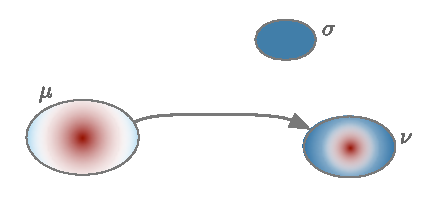
\includegraphics{Metapop_scheme.pdf}
\caption{Three meta-populations $\mu $,$\nu $ and $\sigma $ of different size and infection status.
The infection status is represented by the local color distribution.
The edge $(\mu, \nu )$ indicates migration from $\mu $ to $\nu $.}
\label{fig:metapop_scheme}
\end{SCfigure}

In the context of epidemics every subpopulation has a different infection status, i.e. a distribution of $S$, $I$ and $R$.
Additionally to the local infection model, we add a migration term so that the general form of a meta-population SIR-infection-model for a subpopulation $\mu $ is
\begin{equation}\label{eq:general_metapop_sir}
\frac{dI_\mu }{dt} = R(S_\mu, I_\mu , R_\mu) + M (S_\mu, I_\mu , R_\mu, S_\nu ,I_\nu ,R_\nu, \tau ).
\end{equation}
The first term $R$ in equation \eqref{eq:general_metapop_sir} is a \emph{local reaction} term, while the \emph{migration} $M$ to other subpopulations could depend on the local distribution and the infection status of other subpopulations connected to $\mu $.
Furthermore, the migration between subpopulations could occur on a time-scale $\tau $ different from the time-scale of the local infection.
The impact of these time-scales on disease spread was analyzed in  \citep{cross2005,Balcan:2011gv,Lentz:2012pre}.
We investigate the interplay between network properties and disease outbreaks in section xx. 
%


%\bibliographystyle{apalike}
%\bibliography{/Users/lentz/Documents/GitHub_locals/Thesis/bibliography.bib}
%\end{document}
